\documentclass{beamer}
\usepackage{amsmath, amsfonts, amssymb}
\usepackage{graphicx}
\usepackage{hyperref}
\usepackage{bm}

\renewcommand{\vec}{\bm}
\newcommand{\uvec}[1]{\vec{e}_{#1}}
\newcommand{\td}[2]{\frac{d{#1}}{d{#2}}}					% Total derivative
\newcommand{\pdt}[2]{\frac{\partial{#1}}{\partial{#2}}}	% Partial derivative in first traditional form
\newcommand{\md}[2]{\frac{D{#1}}{D{#2}}}					% Total derivative
\newcommand{\tds}[2]{\frac{d^2{#1}}{d{#2}^2}}
\newcommand{\pdts}[2]{\frac{\partial^2{#1}}{\partial{#2}^2}}

\newcommand{\op}{\prime}
\newcommand{\dive}{\nabla\cdot}

\usefonttheme[onlymath]{serif}

\title{Accretion Discs}
\author{Amey Joshi}
\date{03-Feb-2023}

\begin{document}
\frame{\titlepage}

\begin{frame}
\frametitle{Gravity as an energy source}
\begin{itemize}
\item Physicists of the 19th century believed that the stars are powered by gravity.
\item Gravitational potential energy of the sun is
\begin{equation}\label{e1}
U = -\frac{3}{5}\frac{GM_\odot^2}{R_\odot}
\end{equation}
By \href{https://en.wikipedia.org/wiki/Virial_theorem}{virial theorem} half of it can be radiated. If $L_\odot$ is the sun's 
luminosity then the sun can shine for a time
\begin{equation}\label{e2}
t = \frac{1}{2}\frac{|U|}{L} = \frac{3}{10}\frac{GM_\odot^2}{R_\odot L_\odot}
\end{equation}
\item Using the approximate values $G \approx 7 \times 10^{-11}, M_\odot \approx 2 \times 10^{30}$, $R_\odot \approx 7 \times
10^{8}, L \approx 4 \times 10^{25}$ in SI units we get $t \approx (3/10) \times 10^{16}$ s. A year has approximately $3 \times
10^7$ s. Therefore the sun will shine for $t \approx 100$ million years.
\end{itemize}
\end{frame}

\begin{frame}
\frametitle{Gravity as an energy source}
\begin{itemize}
\item If the sun contracted from $5$ times its current radius, it would have shone for $20$ million years before it got to
today's size.
\item This is surely less than the age of the earth estimated by the 19th century geologists.
\item It was only in the early years of the 20th century that people found alternative source of energy to power stars - nuclear 
reactions.
\item Yet not everything in the universe shines because of nuclear power.
\end{itemize}
\end{frame}

\begin{frame}
\frametitle{Accretion an an energy source}
\begin{itemize}
\item The potential energy of a mass $m$ in the gravitational field of another mass $M$ at a distance $r$ is $GMm/r$.
\item If the potential energy is completely converted to radiation then the energy released per unit mass by accretion by an object 
of radius $R$ and mass $M$ is $GM/R$. If $M \approx M_\odot$ and $R \approx 10$ km, it is $O(10^{16})$ J/kg.
\item Energy released per unit mass by H $\rightarrow$ He reaction is $0.007 c^2$ which is $6 \times 10^{14}$ J/kg.
\item Accretion by compact objects can release tremendous amount of energy. 
\item The next slide shows how accretion is important for compact objects.
\end{itemize}
\end{frame}

\begin{frame}
\frametitle{Accretion versus nuclear energy}
\begin{figure}
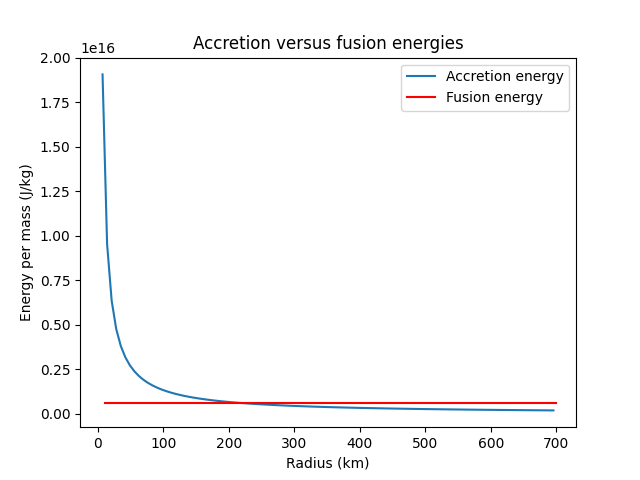
\includegraphics[scale=0.5]{Figure_1.png}
\caption{Energy released per unit mass by accretion and nuclear fusion}
\label{f1}
\end{figure}
\end{frame}

\begin{frame}
\frametitle{Accretion discs}
\begin{itemize}
\item Dense, compact objects were not known in the 19th century.
\item Pulsars, neutron stars, quasars, active galactic nuclei and black holes were all discovered only the last few decades.
\item All of these accrete mass from their surroundings and are sufficiently compact to emit energetic radiation.
\item The idea of accretion of mass by stars preceeded the observation of compact objects. Hoyle, Lyttleton and Bondi considered
the problem of accretion of interstellar material by stars in the late 1930s and early 1940s.
\item In this talk we will review the theory of accretion flows from 1930s up to the recent times.
\end{itemize}
\end{frame}

\begin{frame}
\frametitle{Scheme of the talk}
\begin{itemize}
\item Brief overview of accretion flows.
\item Peculiarity of disc formation.
\item The role of angular momentum.
\item Shakura and Sunyaev model for steady thin discs
\end{itemize}
We will focus on the physical model and not consider the observational details. The goal is to understand how and why are accretion discs formed and to 
consider one simple model that allows us to compute a fundamental observational quantity, the luminosity.
\end{frame}

\begin{frame}
\frametitle{An accretion disc}
We want to understand how such a structure is formed.
%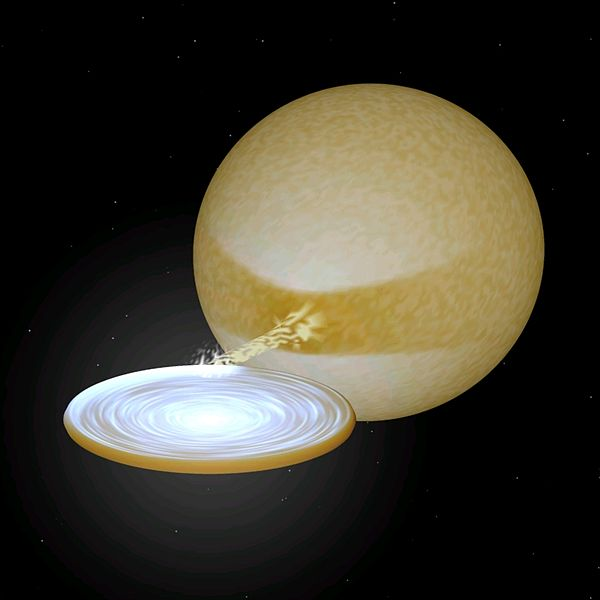
\includegraphics[width=\paperwidth]{600px-Low-mass_X-ray_binary}
\begin{center}
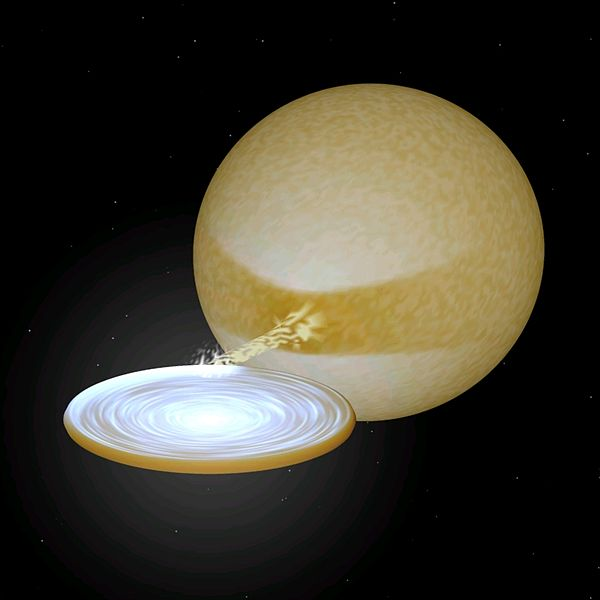
\includegraphics[scale=0.25]{600px-Low-mass_X-ray_binary}
\end{center}
\end{frame}

\begin{frame}
\frametitle{Accretion flow -  moving star}
\begin{itemize}
\item Hoyle and Lyttleton  conjectured the change in radiation because of accreting matter and its impact on the earth's weather. 
\item If the star of mass $M$ moves with a speed $v$ through the interstellar matter then all particles within a distance $s$ of the star's centre
will be trapped in the star's gravitational field if
\begin{equation}\label{e3}
s < \frac{2GM}{v^2}.
\end{equation}
\item They further showed that the rate of accretion is
\begin{equation}\label{e4}
\dot{m} = \frac{4\pi G^2M^2\rho_i}{v^3},
\end{equation}
where $\rho_i$ is the mass density of interstellar matter.
\end{itemize}
\end{frame}

\begin{frame}
\frametitle{Accretion flow - stationary star}
\begin{itemize}
\item Hoyle and Lyttleton's analysis considered the interstellar material to be stationary and a star passing through it. Sir H. Bondi considered the other
extreme in which the star is stationary and it attracts interstellar material from all directions. 
\item In Hoyle and Lyttleton's case accretion happens because of the dynamical effect of the gravitational field on the individual particles of the interstellar
medium.
\item In Bondi's case, the accretion happens because of pressure gradient due to the star's gravitational field. The interstellar medium is treated like an
ideal fluid.

\end{itemize}
\end{frame}

\begin{frame}
\frametitle{Accretion flow - stationary star}
\begin{itemize}
\item The analysis is more complicated than Hoyle and Lyttleton's. The maximum rate of accretion is found to be
\begin{equation}\label{e5}
\dot{m} = \frac{4\pi G^2M^2\rho_\infty \lambda_M}{c_s^3},
\end{equation}
where
\begin{itemize}
\item $\rho_\infty$ is the density of the interstellar material at a great distance from the star,
\item $c_s$ is the speed of sound at a great distance from the star and
\item $\lambda_M$ is a function of $\gamma$, the adiabiatic constant of the gas. (Ratio of the two specific heats.) 
\begin{equation}\label{e6}
\lambda_M = \left(\frac{1}{2}\right)^{(\gamma+1)/(2(\gamma-1))}\left(\frac{5-3\gamma}{4}\right)^{-(5-3\gamma)/(2(\gamma+1))}.
\end{equation}
\end{itemize}
\item The flow is considered to be adiabatic, that is, $\gamma \ne 1$.
\end{itemize}
\end{frame}

\begin{frame}
\frametitle{Accretion flows}
\begin{itemize}
\item Neither of the flows considered so far result in an accretion disc.
\item Hoyle and Lyttleton's case results in accretion of matter on the 'front side' of the star.
\item Bondi's case results in spherically symmetric attrition.
\item Disc formation requires a different physical setup. It needs a pair of bodies one of which is large and gaseous and the other a compact object.
\begin{itemize}
\item The flow is \textbf{not} isotropic.
\item The fluid carries the angular momentum of its source.
\end{itemize}
\item The flow occurs because of the instability at the lagrangian point $L_1$.
\end{itemize}
\end{frame}

\begin{frame}
\frametitle{Accretion flow - binary system}
\begin{itemize}
\item Consider two bodies of masses $m$ and $M \gg m$ at positions $\vec{r}$ and $\vec{R}$ respectively.
\item We define the lagrangian sphere of a body as the region around it where its gravitational field dominates every other. Let $S_m$ and $S_M$ be the
lagrangian spheres of the two bodies. They touch each other at the lagrangian point $L_1$.
\item $L_1$ being an unstable point, a mass at $L_1$ will readily slip into either $S_m$ or $S_M$. As $M \gg  m$, it is more likely to slip into $S_M$.
\item If the matter in $S_m$ was moving randomly then it will have angular momentum in all directions.  Therefore, matter leaking from $S_m$ into $S_M$
at $L_1$ will also be randomly oriented and will result in a spherical cloud of accretion around $M$.
\item Yet, we know that a disc is formed. Why? How?
\end{itemize}
\end{frame}

\begin{frame}
\frametitle{Accretion flow - binary system}
\begin{itemize}
\item It can be shown that a rotating mass of a fluid has the least energy when it rotates like a rigid body. That is, the entire mass of the fluid has a uniform
angular velocity $\vec{\omega}$.
\item The matter leaking into $S_M$ has its angular momentum vector along the same direction. (In reality, in a narrow cone around axis of
rotation of $m$.). 
\item This leads to the formation of a disc like flow around $M$. The thickess of the disc is proportional to the semi-angle of the cone which confines all
the angular momenta.
\item This tells us why a disc is possible but we still don´t know why mass gradually moves towards $M$. Why does the mass not confine itself to the inner
surface of $S_M$, the lagrangian sphere of $M$.
\end{itemize}
\end{frame}

\begin{frame}
\frametitle{Accretion flow - binary system}
\begin{itemize}
\item Consider a mass $\delta m$ moving in the gravitational field of $M$. It can be shown that the energy of $\delta m$ is the least when 
\begin{itemize}
\item it has no radial motion. That is, the orbit is circular,
\item its specific energy is given by
\begin{equation}\label{e7}
e = \frac{h^2}{2r} - \psi(r, 0),
\end{equation}
where $h$ is the specific angular momentum, $r$ the radial distance and $\psi$ the gravitational potential that depends on $r$ and $z$. (It does not depend on
the angle $\theta$; we are using cylindrical coordinates here.)
\item its angular speed is
\begin{equation}\label{e8}
\omega = \frac{\partial e}{\partial h}.
\end{equation}
\end{itemize}
\item What is the minimum energy state for two such masses $\delta m_1$ and $\delta m_2$?
\end{itemize}
\end{frame}

\begin{frame}
\frametitle{Accretion flow - binary system}
\begin{itemize}
\item If the two masses do not interact then their minimum energy configurations are the same as if they were isolated. But they do interact!
\item They can exchange energy and angular momentum. If they are fluids they can also exchange mass.
\item It can be shown that the energy is minimised if:
\begin{itemize}
\item Mass is transferred inwards.
\item Angular momemtum is transferred outwards.
\end{itemize}
\item In this case $\omega$ is a function of $r$. Accretion flows have shear stress in the tangential direction. Viscous stress results in a dissipation of energy
resulting in the matter flowing further inward. 
\item Much of the matter travels inwards but a little part of it orbits at increasingly large radius and carries most of the angular momentum with it.
\end{itemize}
\end{frame}

\begin{frame}
\frametitle{Steady thin discs - Shakura and Sunyaev model}
\begin{itemize}
\item A disc is thin if its height $h$ is much smaller than its radius. It is steady if the velocity of its flow is independent of time. (Steady $\ne$ stationary.)
\item It can be shown that the pressure is negligible as compared to gravitational attraction for a flow in a steady, thin disc.
\item Further, the state of the discs is governed by
\begin{eqnarray}
\pdt{\rho}{t} + \frac{1}{r}\frac{\partial}{\partial r}(r\rho v_r)  &=&  0 \label{e9} \\
\frac{\partial}{\partial t}(r^2\sigma\omega) + \frac{1}{r}\frac{\partial}{\partial r}(r^3\sigma v_r\omega) &=&
\frac{1}{r}\frac{\partial}{\partial r}\left(\sigma\nu r^3\pdt{\omega}{r}\right) \label{e10}
\end{eqnarray}
These are the balance equations of mass and 'angular momentum surface density'. In equation \eqref{e10}, $\sigma$ is the surface mass density, $\nu$ the 
kinematic viscosity and $\omega$ is the angular speed.
\end{itemize}
\end{frame}

\begin{frame}
\frametitle{Steady thin discs - Shakura and Sunyaev model}
\begin{itemize}
\item In steady state, the time derivatives vanish and the two equations give
\begin{eqnarray}
r\rho v_r &=& c_1 \label{e11} \\
r^3\sigma\left(v_r\omega - \nu\pdt{\omega}{r}\right) &=& c_2, \label{e11a}
\end{eqnarray}
where $c_1$ and $c_2$ are constants.
\item We can show that
\begin{eqnarray}
c_1 &=& -\frac{\dot{m}}{2\pi} \label{e12} \\
c_2 &=& -\frac{\dot{m}}{2\pi}\sqrt{GMr_\star} \label{e13}
\end{eqnarray}
where $\dot{m}$ is the rate of accretion of mass and $r_\star$ is the radius at which the flow rotates rigidly. (It is the value of $r$ for which 
$d\omega/dr=0$.)
\end{itemize}
\end{frame}

\begin{frame}
\frametitle{Steady thin discs - Shakura and Sunyaev model}
\begin{itemize}
\item This analysis leads to the following conclusions:
\begin{itemize}
\item The kinematic viscosity depends on $r$,
\begin{equation}\label{e14}
\nu = \frac{1}{3\pi\sigma}\left(1 - \sqrt{\frac{r_\star}{r}}\right)\dot{m}.
\end{equation}
\item The rate of energy emitted by the disc is
\begin{equation}\label{e15}
Q = \frac{3GM\dot{m}}{4\pi r^3}\left(1 - \sqrt{\frac{r_\star}{r}}\right).
\end{equation}
\item The luminosity of the disc is
\begin{equation}\label{e16}
L = \int_{r_\star}^\infty\int_0^{2\pi} QRrdrd\theta = \frac{GM\dot{m}}{2r_\star}.
\end{equation}
\end{itemize}
\end{itemize}
\end{frame}

\begin{frame}
\frametitle{Steady thin discs - Shakura and Sunyaev model}
\begin{itemize}
\item At the edge of the disc where $r = r_\star$ and where the boundary between rigid rotation and otherwise lies, the gravitational
potential energy of the compact object is $-GM/r_\star$. If $\dot{m}$ is the rate of accretion then $-GM\dot{m}/r_\star$ is the
rate at which energy is acquired by the compact object and its disc. Equation \eqref{e16} suggests that half of it is
radiated away as the disc's luminosity.
\end{itemize}
\end{frame}
\end{document}
